\section{Durchführung}
\label{sec:Durchführung}
Es soll zunächst die Zeitabhängigkeit der Amplitude untersucht werden und daraus der effektive Dämpfungswiederstand $R_{eff}$ bestimmt werden.
Dazu wurde eine Schaltung \autoref{abb:5a} entsprechend aufgebaut und der Schwingkreis zu einer gedämpften Schwingung angeregt.
Es wurde der kleinere der in der Schaltung eingebauten Wiederstände verwendet und die Spannung sowie das Oszilloskop so eingestellt,
dass die Amplitude der gedämpften Schwingung um ca. den Faktor 3-8 abgenommen hat bevor diese erneut beginnt.
\begin{figure}[H]
    \centering
    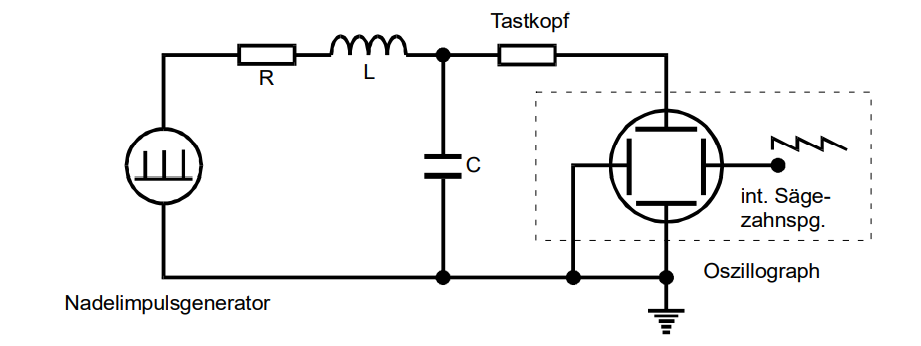
\includegraphics[scale=0.8]{content/5a.png}
    \caption{Die für 5a verwendete Schaltung. \cite{sample}}
    \label{abb:5a}
\end{figure}
\noindent Außerdem soll der Dämpfungswiederstand $R_{ap}$ bestimmt werden, bei dem der aperiodische Grenzfall vorliegt.
Dafür wurde eine Schaltung nach \autoref{abb:5b} verwendet und der verstellbare Wiederstand so eingstellt, dass sich
so gerade eben kein Überschwingen zeigt, indem dieser von seinem Maximalwert langsam verringert wurde.
\begin{figure}[H]
    \centering
    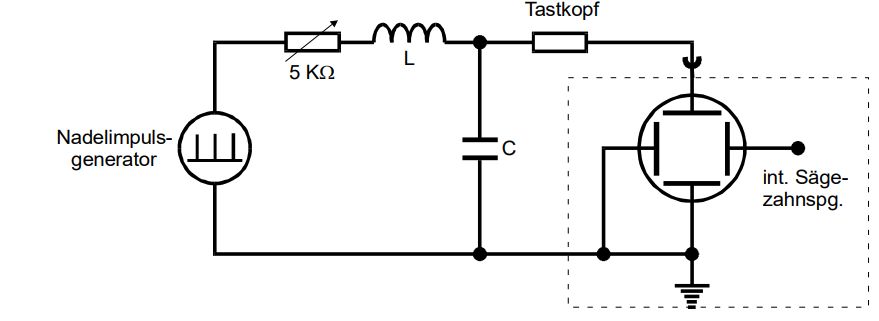
\includegraphics[scale=0.8]{content/5b.png}
    \caption{Die für 5b verwendete Schaltung. \cite{sample}}
    \label{abb:5b}
\end{figure}
\noindent Zuletzt sollen die Frequenzabhängigkeit der Kondensatorspannung und der Phase zwischen Erreger- und Kondensatorspannung
am Serienresonanzkreis untersucht werden. Die verwendete Schaltung entspricht der in \autoref{abb:5cd} dargestellten. Dabei wurden
Wertepaare der Erregerspannung, Kondensatorspannung und den Parametern a und b nach \autoref{abb:5d} zu verschiedenen Frequenzen vom Oszilloskop
entnommen.
\begin{figure}[H]
    \centering
    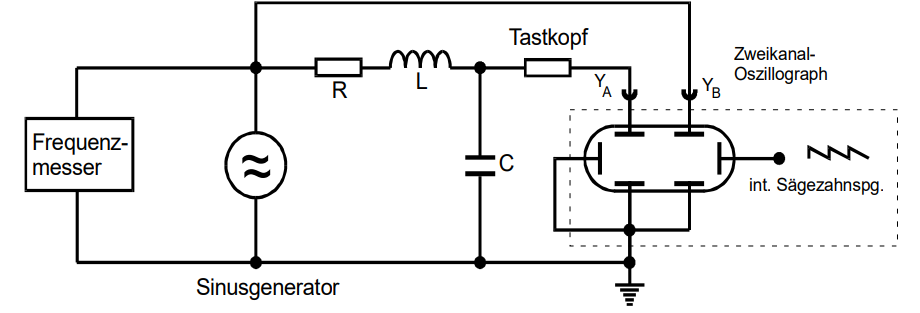
\includegraphics[scale=0.8]{content/5cd.png}
    \caption{Die für 5c und 5d verwendete Schaltung. \cite{sample}}
    \label{abb:5cd}
\end{figure}
\begin{figure}[H]
    \centering
    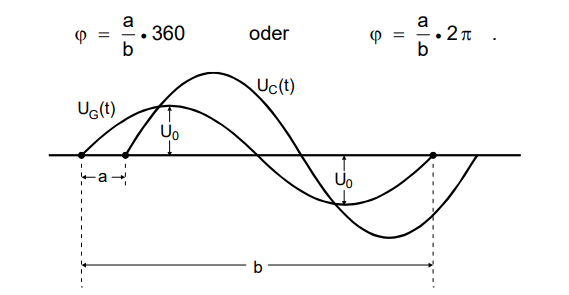
\includegraphics[scale=1]{content/5d.png}
    \caption{Die Phasenverschiebung der Erreger- und Kondensatorspannung. \cite{V353}}
    \label{abb:5d}
\end{figure}
